% 标单百分号的注释,如本句所示。是原本模板注释
%%% 标三个百分号的注释,如本句所示。是辅助使用者理解的指导性演示,以“-BEGIN”与“-END”进行标记代码的起始位置和结束位置

%%% 与此同时,本文档作为包含子文件与分页符演示,其余功能演示内容详见 ./section/2.3.1_步兵机器人.tex 文档

% 引入导言区配置文件

%%% 包含子文件演示-BEGIN
% 文档全局设定与引入必要宏包

\documentclass[a4paper, twoside, zihao=-4, sub3section]{article}
\usepackage[hmargin=0.79in, top=0.95in, bottom=1.13in]{geometry}
\geometry{headsep=0.14in, footskip=0.47in}

\usepackage{pdfpages}
\usepackage{amsmath}
\numberwithin{figure}{section}
\usepackage{fancyhdr}

\usepackage{graphicx}
\usepackage{float}

\usepackage{ltxtable}
\usepackage{colortbl}
\usepackage{multirow}
\usepackage{graphicx}

% 字体配置

\usepackage[UTF8, heading=true]{ctex}
\setmainfont{Arial}
\setsansfont{Arial}
\setCJKmainfont[AutoFakeBold, AutoFakeSlant]{SimSun.ttc}
\setCJKsansfont[AutoFakeBold, AutoFakeSlant]{SimHei.ttf}

% 段落格式配置

\linespread{1.62}
\setlength{\parskip}{5pt}

% 目录配置

\usepackage[titles]{tocloft}
\usepackage{hyperref}
% 去除引用红框,改变颜色
\hypersetup{colorlinks=true,linkcolor=black}
% 重新定义目录的标题样式
\renewcommand*\contentsname{\hfill \color{black}\zihao{-2}\textbf{目录} \hfill}
% 设置点间距
\renewcommand\cftdotsep{0.1}
\renewcommand\cftsecdotsep{\cftdotsep}
\CTEXsetup[name={,.}]{section}
% 调节缩进
\setlength{\cftsubsecindent}{1em}
\setlength{\cftsubsubsecindent}{3em}
% 调节编号宽度
\setlength{\cftsecnumwidth}{14pt}
\setlength{\cftsubsecnumwidth}{20pt}
\setlength{\cftsubsubsecnumwidth}{30pt}
% 调节行距
\setlength{\cftbeforesecskip}{0pt}

% 标题配置

\usepackage{xcolor}
\newcommand{\titlecolor}{\color[RGB]{51, 51, 153}}
\usepackage{titlesec}
\titleformat{\section}
  {\titlecolor\zihao{2}\bfseries}
  {\thesection.}{0.5em}{}
\titleformat{\subsection}
  {\titlecolor\zihao{-2}\bfseries}
  {\thesubsection}{0.5em}{}
\titleformat{\subsubsection}
  {\titlecolor\zihao{3}\bfseries}
  {\thesubsubsection}{0.5em}{}
% 四级标题
\setcounter{secnumdepth}{4}
\titleformat{\paragraph}
  {\titlecolor\zihao{-3}\bfseries}
  {\theparagraph}{0.5em}{}

% 表格样式配置

\definecolor{tabhdcolor}{hsb}{0, 0, 0.72353}
\definecolor{gndcolor}{hsb}{0, 0, 0.96}
\AtBeginEnvironment{longtable}{\sffamily}
\renewcommand{\arraystretch}{1.1}
%%% 包含子文件演示-END
%%% 包含子文件,相当于把被包含的文件全部内容复制粘贴到此处
\usepackage{enumitem}
\usepackage{amssymb}
\usepackage{pifont}
\usepackage{graphicx}
\usepackage{array}
\usepackage{longtable}
\usepackage{tabularx}
% 文档内容-BEGIN
\begin{document}

    % 引入封面
    % 封面

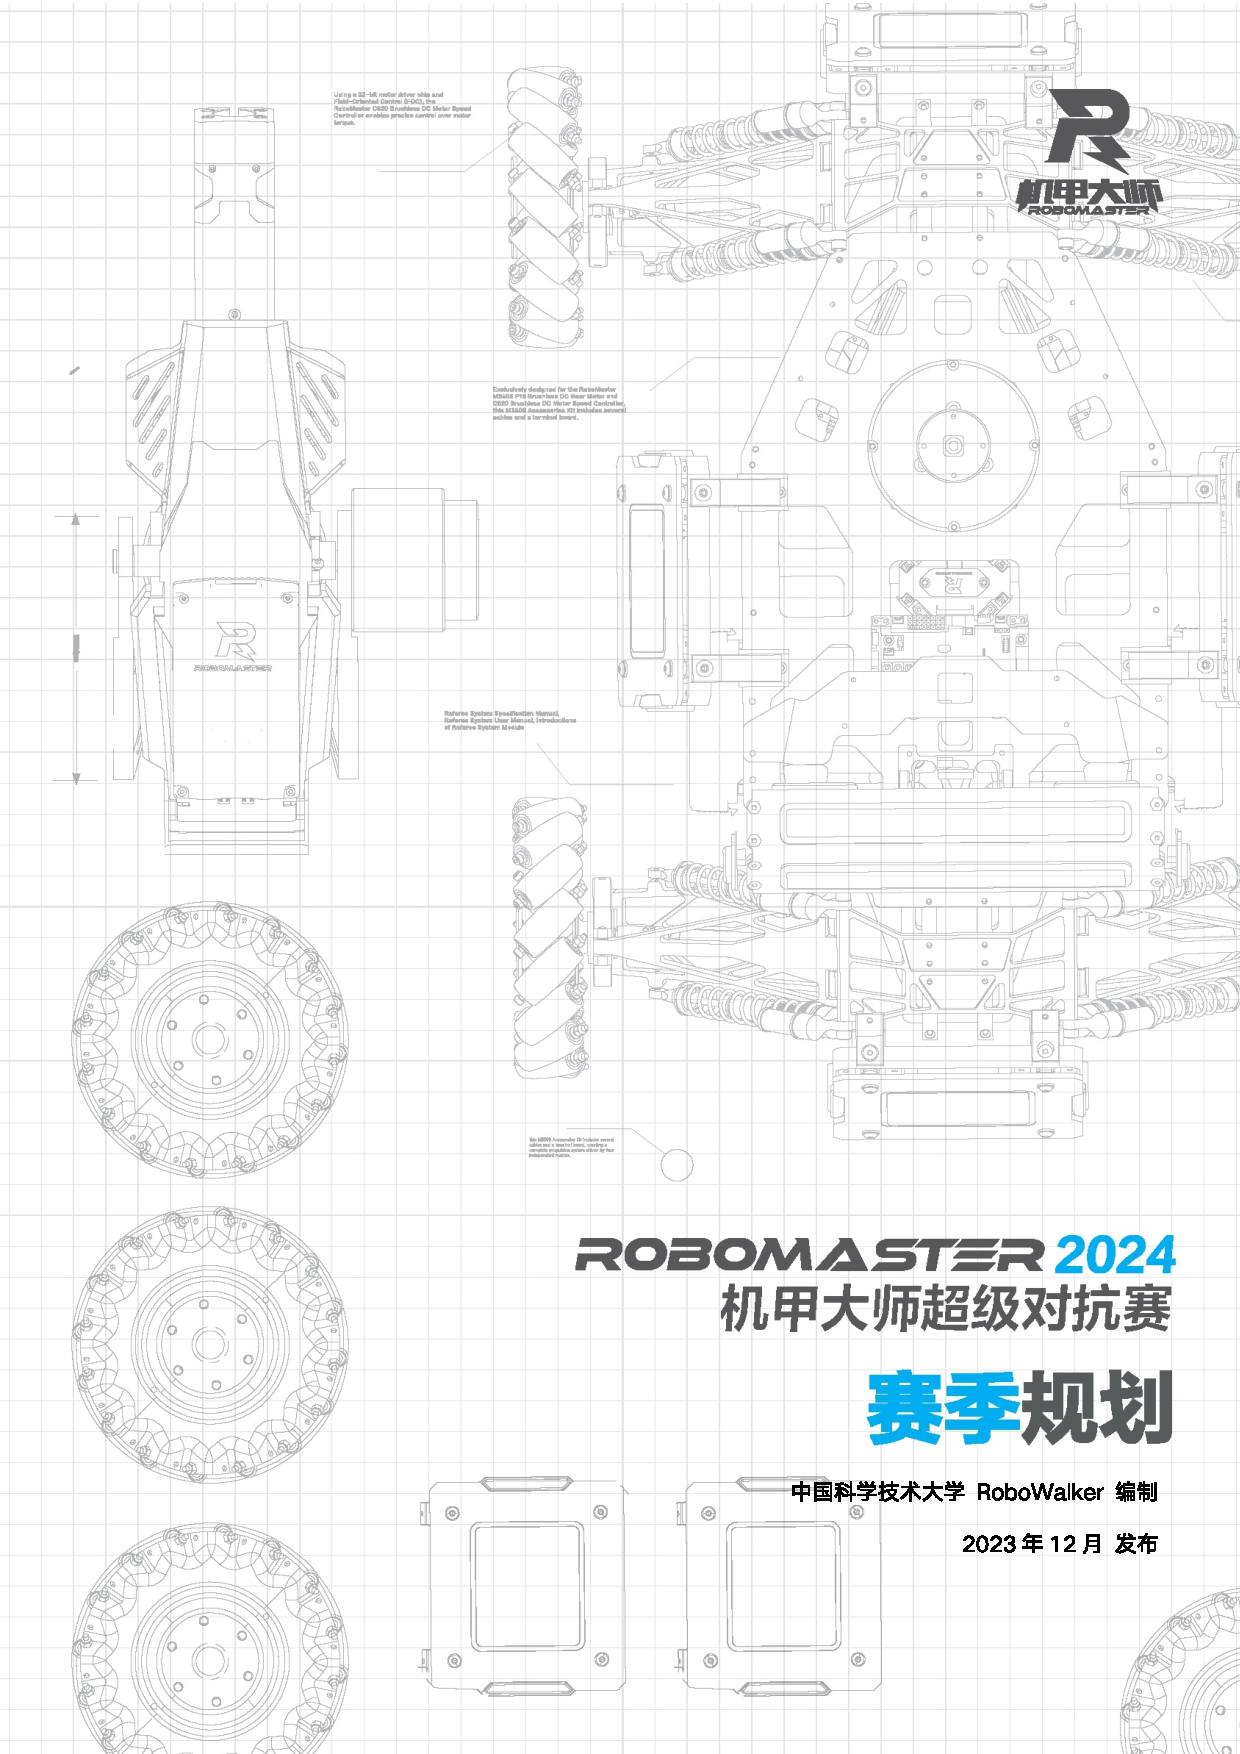
\includepdf{section/cover1.pdf}

% 编码页数从1开始
\setcounter{page}{1}

% 页眉页脚
\pagestyle{fancy}
\fancyhf{}
\fancyhead[EL, OR]{
  
\includegraphics[height=0.15in]{figure/header_img.png}
}
\fancyfoot[EL]{
  \zihao{-4}\thepage
  \hspace{0.4cm}
  \raisebox{.15ex}{
    \color{gray}{
      \zihao{-5}© 2024 \ 大疆创新 \ \ 版权所有
    }
  }
}
\fancyfoot[OR]{
  \raisebox{.15ex}{
    \color{gray}{
      \zihao{-5}© 2024 \ 大疆创新 \ \ 版权所有
    }
  }
  \hspace{0.4cm}
  \zihao{-4}\thepage
}

% 目录
\begin{center}
  \zihao{5}\tableofcontents
\end{center}

\newpage
    
    \section*{前言}

\addcontentsline{toc}{section}{前言}
    
    \noindent
    本报告由深圳技术大学悍匠战队编制,适用于RoboMaster 2025机甲大师超级对抗赛。主要撰写人员包括:
    
    \noindent
    \LTXtable{\textwidth}{table/0_writersList.tex}
    
    %%% 分页符演示-BEGIN
    \newpage
    %%% 分页符演示-END
    %%% 分页符,相当于从此处开辟新的一页,无论上一页内容是否凑够一页,都会从新的一页开始
    
    \section{团队目标}


    \subsection{团队目标概括}

        深圳技术大学悍匠战队始建于2019年,至今已有5年的备赛经验,自22赛季首次踏入超级对抗赛赛场后,均未能在区域赛的小组中出现,未能实现赛季成绩的进一步突破。\par
        对此,我们剖此往届赛季备赛中出现的管理和技术层面的不足之处,复盘反思与强队交手的经历,25赛季我们战队的比赛目标是晋级全国赛。\par
        为实现这个多年来的愿望,在25赛季中加强进度监管、在原有基础之上细微调整和优化、备赛过程中侧重于测试、进一步体系化传承资料和财务等各方面流程、引导队员探索技术背后的原理;加强队伍文化建设,提高队员比赛积极性和参与感,营造追求极致、患难与共的团队氛围,将生而无畏,精益求精的团队理念贯彻到每个战队成员。\par

        \subsubsection{团队实际情况}

            \paragraph{队伍可用资源}

                得益于学校和学院的大力支持,本赛季战队在资金、研发场地等方面比较充足。本赛季战队的资金来源主要有以下几个方面:上赛季剩余的耗材费、加工费等,2025年学院竞赛专项经费、实验室运行费用等多项经费约30万元。\par
                战队共有研发装配实验室3个,用于加工及物料存放的实验室1个,并配有一个约100平方测试场地可以放置1个联盟赛3V3对抗赛场地或1/4个超级对抗赛场地。\par
                战队拥有多台 3D 打印机,台钻,切割机,磨砂机等设备用于加工研发,拥有电子白板、打印机等设备满足队内授课、开会、成果展示等需求,配备了云台相机、单反相机、无人机等设备,能够满足战队宣传需求。此外通过老队员的资助实验室还配备了冰箱、制冰机等设施,提高队员生活质量。整体来看,我们战队的资源相对充足,能够满足战队的研发需求。\par
                目前我队拥有团队成员共 80 余人,根据我校课程设置、实习安排等实际情况,我们队伍的人员构成主要如下:大二队员是队伍的主干力量,需要完成本赛季各兵种的基础研发装配调试迭代工作,是比赛的主要参与者;大三与大四留队队员参赛经验较为充足,但因为自身学业与未来就业原因,偶尔会在队内对队伍进行指导,同时根据队员自身情况,进行相应技术点的研究与突破。大一队员作为梯队成员,经行比赛基础基础技能学习,完成各组队内考核的任务,进行各类基础模块建设与调试,同时为鼓励大一成员积极参与,研发创新,表现优异者可作为正式队员参赛。\par
                关于技术积累部分,经过上赛季的转变,传承下来的资料相较完整和体系化,在25赛季将继续推进各组文本、视频等形式的技术传承。我们队内主要的技术资源获取途径有邀请老队员回来对技术研究可行性分析、老队员留下的技术文档、公开的论文资料、工业界成熟的技术下放、组织与其他队伍的线下技术交流、RoboMaster论坛各队开源技术分享,以及各RM交流群的技术交流。\par

        \subsubsection{本赛季要完成的基础内容及进阶优化内容}

                经过过去几年各赛季的复盘和反思,历史的备赛策略过于激进、新赛季多次推翻旧赛季千辛万苦打下的基础,赛季初踌躇满志、备赛时忙不过来、缺乏明确的测试计划、赛场上稳定性欠佳。队员们普遍缺乏科学合理的设计和控制策略,这反映了主流的以项目驱动发展的学习路线无法兼顾犄角旮旯的知识空缺,队员们往往只能够解决具体的工程实践问题,而对技术背后的原理漠不关心,这是队员和队伍谋求长远发展无法忽视的阻碍。\par
                稳定性:在设计时,需要充分考虑模块的使用场景,在结构和配件材料选型上尽量做到合理;在装配时选择正确的零件,在交付下一环节前完成可用性和强度的检查,并及时记录缺陷以便于下一版本迭代;注意线路的布置合理与线束的物理保护,对可能磨损线材的地方加强保护,留下记录,并在下一版本设计上做出调整。此外,只有长期高强度的测试能够检验稳定性是否良好,在缺乏科学的分析能力的情况下也只有测试能够暴露出不稳定缺陷。\par
                设计指标与测试计划:在机器人研发的初始节点定下机器人性能指标并根据制定相应的调试测试计划,在队里进度管理系统中留下记录。测试也不止步于记录,需要将大量的测试数据汇总后分析成因。\par


            


    %\input{section/1.1.1_teamReality}

    %\input{section/1.1.2_unfinishedContent}

    \subsection{各方向上的目标}

    \subsubsection{目标成绩}

        在比赛成绩上,由于我们战队已经有 5 次参加 RoboMaster 比赛的经验,并有两次成功参加超级对抗赛的经验,战队内经过全体讨论决定,本赛季希望能够进入全国赛。\par

    \subsubsection{任务进度管理制度}

        在赛季的各个阶段制定各兵种的整体任务进度安排,并将阶段性任务记录在飞书云文档,规定每个任务结束时间,每周定期由项目负责人核实验收上周任务完成情况并对遇到的问题进行总结并制定本周的工作安排,队长及项管参与每周各组工作安排会议,保证每个项目所需资源落实到位,进度情况健康。任务进度管理数字化记录,在项目管理系统上登记每周任务并实时更新任务状态,对进度情况不健康的项目做出及时调整。\par

    \subsubsection{队员管理制度}

        结合队员个人课程表情况对队员在实验室到岗研发时间有所要求,完善实验室考勤请假制度,考虑到学校人数越来越多,我们考虑对人员的要求要精益求精,整顿队风,对比赛参与度不高,研发积极性差,工作效率低效的队员作警告清退处理。同时提高实验室成员的责任意识,爱护实验室资产与环境,并制定了相应的奖惩制度,加强对梯队队员的培养。\par

    \subsubsection{物资管理制度}

        构建数字化流程化物资购买管理制度,增强对物资购买的流程审核及记录,提高现有资源利用率,减少不必要的浪费,对高价值物资如电机进行出入库登记处理,物资领用责任到人,对于由于低级错误或者恶意损坏物资的成员实行罚款制度。\par

    \subsubsection{新人培养体系}

        构建数字化流程化物资购买管理制度,增强对物资购买的流程审核及记录,提高现有资源利用率,减少不必要的浪费,对高价值物资如电机进行出入库登记处理,物资领用责任到人,对于由于低级错误或者恶意损坏物资的成员实行罚款制度。\par

    \subsubsection{管理流程改变}

        本赛季的管理方式继续沿用上赛季队长,项管主导项目方向,各技术组组长评估技术可行性,各车组负责人主导研发方向的形式,主要流程为:队长项管制定各车组的需求,技术组长分析技术可行性,的出最终需求结论,由车组负责人制定研发方向,再由技术成员讨论技术细节。\par

    \subsubsection{技术传承建设}

        在研发调试过程中遇到缺陷或陷阱及时记录,撰写“警钟长鸣”文档,对每个新研发的技术点留下相应的技术文档。在赛季结束都需要撰写自己负责部分的技术文档(包括已实现的技术细节和未实现的预研资料),安排相关负责人跟进文档进度。\par

    %\input{section/1.2.1_targetAchievement}

    %\input{section/1.2.2_taskSchedule_management}

    %\input{section/1.2.3_teamMember_management}

    %\input{section/1.2.4_teamMaterial_management}

    %\input{section/1.2.5_newcomerTraining}

    %\input{section/1.2.6_managementProcess}

    %\input{section/1.2.7_technologyInheritance}

    \subsection{技术突破}
    
    \newpage
    
    \section{项目分析}

    
    \subsection{上赛季项目分析经验}

    
    \subsection{新赛季规则解读}

    
    \subsection{研发项目规划}

    
    %%% 本文档作为功能演示

\subsubsection{步兵机器人}

    %%% 长段演示-BEGIN
    第一段第一段第一段第一段第一段第一段第一段第一段第一段第一段第一段第一段第一段第一段第一段第一段第一段第一段第一段第一段。\par
    
    第二段第二段第二段第二段第二段第二段第二段第二段第二段第二段第二段第二段第二段第二段第二段第二段第二段第二段第二段第二段。\par
    
    第三段第三段第三段第三段第三段第三段第三段第三段第三段第三段第三段第三段第三段第三段第三段第三段第三段第三段第三段第三段。\par
    %%% 长段演示-END

    \paragraph{需求分析}
    
        %%% 有序列表演示-BEGIN
        \begin{enumerate}
            \item 需求1。
        
            \item 需求2。
        \end{enumerate}
        %%% 有序列表演示-END
    
        %%% 插入公式演示-BEGIN
        \begin{align*}
            \Vec{OP} &= \frac{1}{2} ( \Vec{OB} + \Vec{OD} ) = \frac{1}{2} ( \Vec{OA} + \Vec{AB} + \Vec{OE} + \Vec{ED} ) \\
            |PC| &= \sqrt{|BC|^2 - |BP|^2} \\
            \Vec{OC} &= \Vec{OP} + |PC|\hat{PC} , ~{where}~ \hat{PC} \perp \hat{BP} \\
            \Rightarrow l &= |OC| \\
            \Rightarrow \varphi_0 &= \pi + \arctan(z_C, x_C) \\
        \end{align*}
        %%% 插入公式演示-END
        %%% 具体公式具体分析,公式排版很复杂,是一门学问
    
    \paragraph{设计思路}
        
        %%% 插入图片演示-BEGIN
        \begin{figure}[H]
            \centering
            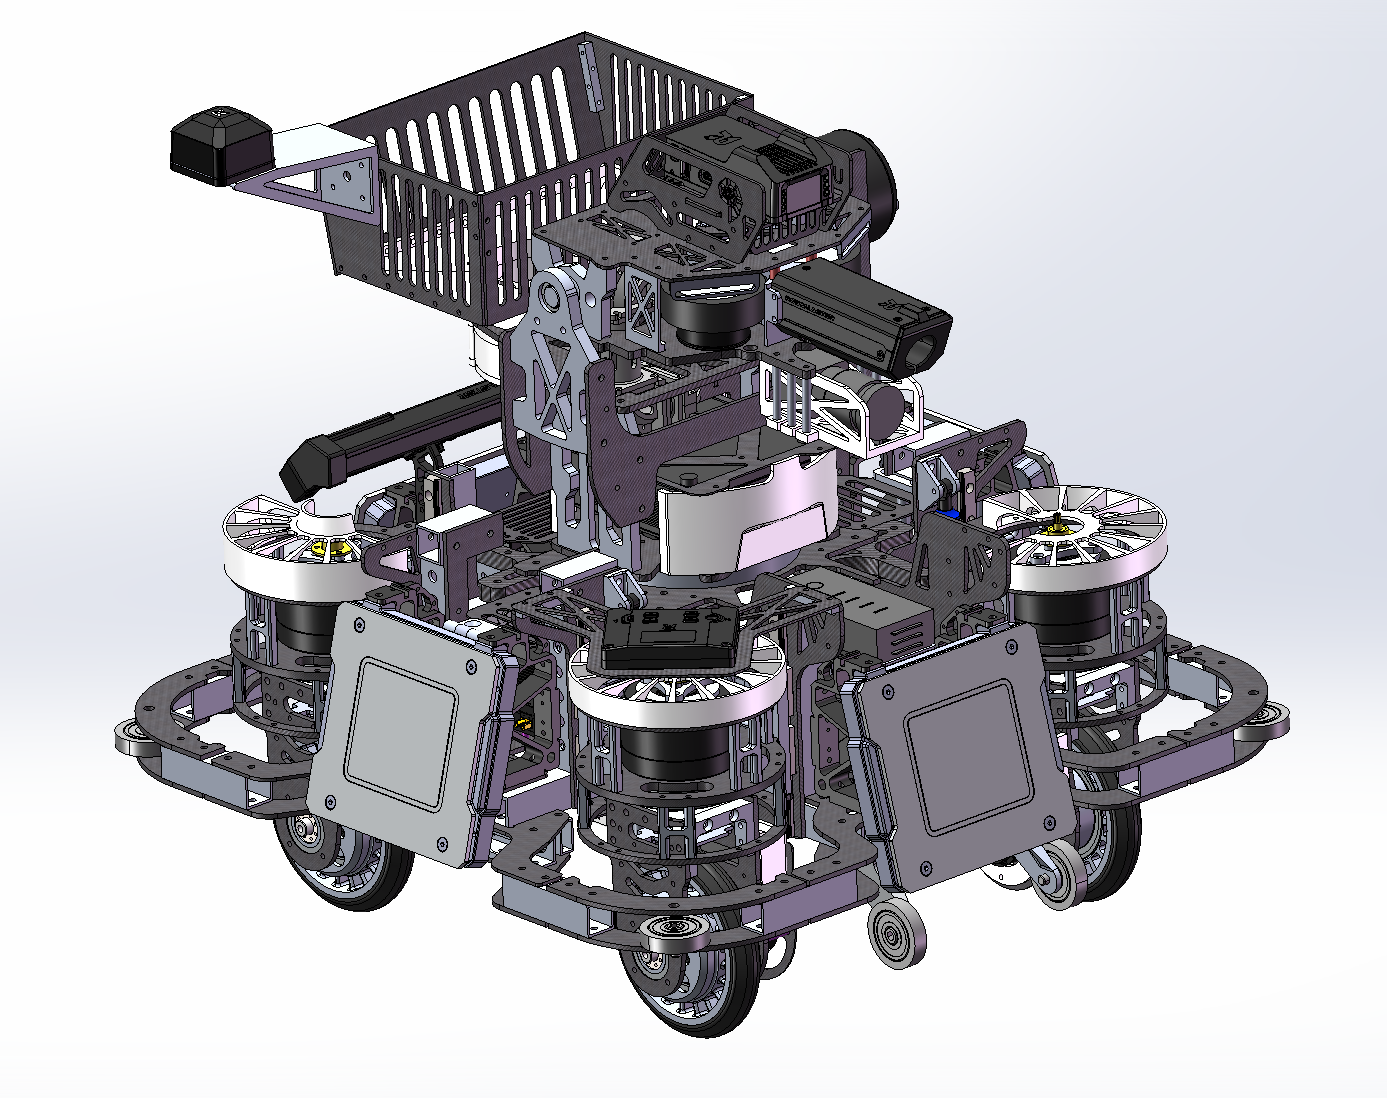
\includegraphics[height=0.35\textwidth]{figure/2_test1.png}
            \hspace{0.5em}
            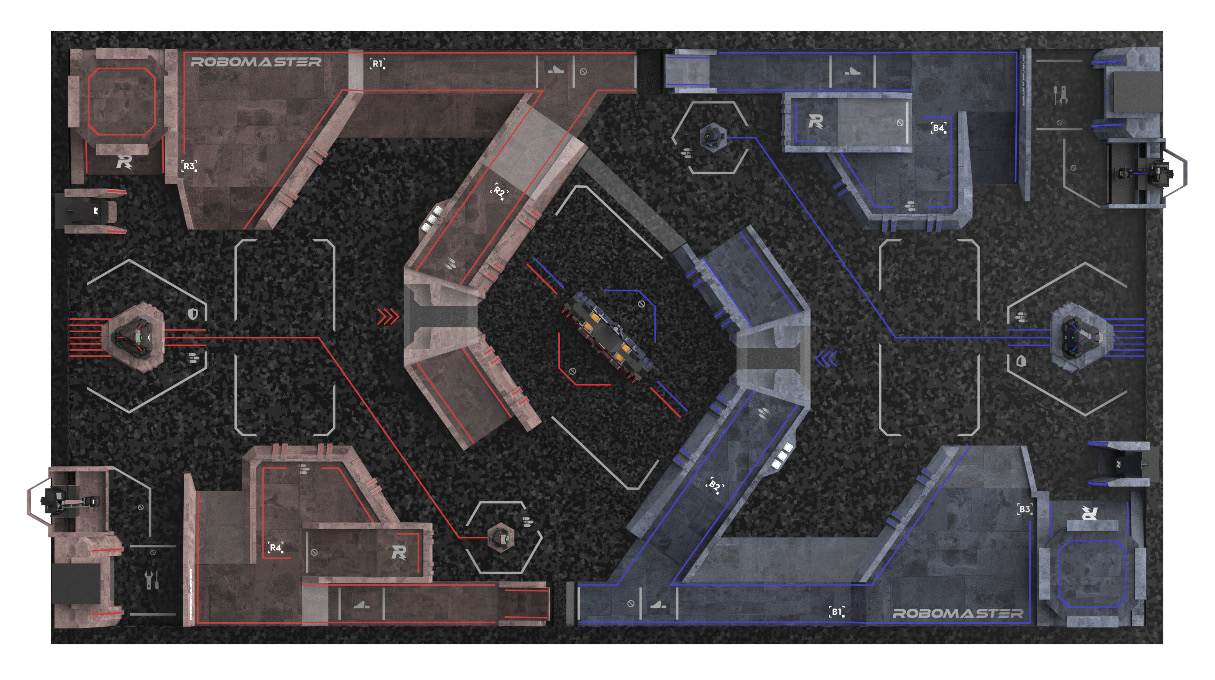
\includegraphics[height=0.35\textwidth]{figure/2_test2.png}
            \label{fig:test}
        \end{figure}
        %%% 插入图片演示-END
        %%% 图片居中放置
        %%% 该图片存储路径为 ./figure/2_test1.png 以及 ./figure/2_test2.png两张图
        %%% \label表示的是该图坐标位置,可以由其他地方引用跳转

    \paragraph{任务安排}
    
        %%% 插入图片引用演示-BEGIN
        点击此处跳转到四舵轮底盘图片处:
        \ref{fig:test}
        %%% 插入图片引用演示-END
        %%% fit:后面的内容为图片对应的label
        
        点击此处跳转到大疆官方比赛配件网站:
        %%% 插入网址引用演示-BEGIN
        \href{https://www.robomaster.com/}{RM官网}
        %%% 插入网址引用演示-END

        %%% 无需缩进的时候可以加一句整个
        \noindent
        
        %%% 插入表格演示-BEGIN
        \LTXtable{\textwidth}{table/2_插入表格示例.tex}
        %%% 插入表格演示-END
        %%% 该表格存储路径为 table/2_插入表格示例.tex ,表格相关代码的具体内容可以打开该文件查看
    
    \subsubsection{英雄机器人}

    \paragraph{规则分析}

        \setlist[itemize]{label=\raisebox{-1.2ex}{\scalebox{3}{$\textbullet$}}}

        \begin{itemize}
            \item 新赛季对英雄性能体系作出较大改变,发射机构为默认模式,发射速度上限默认为16m/s, 相较于上赛季的弹速优先发射机构,本赛季的发射机构的枪口热量上限和枪口热量每秒 冷却值都提升了,跟上赛季爆发优先的发射机构的初始数值一致,相当于本赛季默认的 发射机构结合了上赛季爆发优先和弹速优先的优点,有利于英雄机器人在短时间内持续 进行有效输出,英雄机器人的输出能力会得到提高。
            \item 新增雷达机制被对方雷达机器人标记进度大于100时,对方攻击效益加增百分之十五, 要求英雄机器人机动性更强,躲避对方集火攻击。
            \item 新赛季增益点机制中,相较于上赛季的增益点增益都是单数值,本赛季增益点增益值随 时间,在比赛开始2-3分钟、3-5分钟、5-7分钟时,占领己方基地增益点或高地增益点 深圳技术大学 悍匠  或飞坡增益点或前哨站增益点的机器人,分别可获得2、3、5倍枪口热量冷却增益,比赛 开始前两分钟无冷却增益,前期在R2高地上不能短时间内攻破对方前哨战,因此本赛季 英雄机器人前期攻打前哨战保险方案是在公路区或是R3高地对前哨战进行击打,这对英 雄机器人命中率有了更高的要求。
            \item 新赛季中R3梯形高地的变化使得英雄机器人在此处增益点的机动性更强,利于英雄机器 人在面对对方步兵机器人的追捕;并且,新赛季中R2环形高地新增隧道地形,机器人可 通过该隧道从基地区突击至荒地区;公路区的台阶高度降低有利于降低英雄机器人下台 阶卡住的概率;台阶高度的降低也降低了英雄机器人上台阶的难度,研发可上台阶的机 构也成为本赛季的一大技术难点。
            \item 新赛季中新增半自动控制模式,选手端将会显示与云台手近似的大地图界面,操作手可 以通过在大地图界面内点击的方式向所控制的机器人发送信息。并且在该种模式下机器 人获得较大增益,相较于手动操作,有 50\%的经验增益。但需要英雄机器人具有建图和 导航能力,还需要有精准的自瞄能力,对英雄机器人各个方面提出了更高的要求。
            \item 经验体系:新增发射弹丸即可获得经验机制;对机器人、基地和前哨站造成伤害即可获得 经验机制;删除随时间自然增长经验值机制;击毁机器人时击毁者和助攻者经验值获取 计算方式发生改变;新增狙击伤害获得经验值机制和首次获得飞坡增益获取 300 经验值 机制。总之,在战术上英雄机器人应主动出击,增强飞坡能力,快速精准狙击敌方机器人 和基地、前哨站,以较快获取经验升级。
        \end{itemize}
    
    \paragraph{策略战术}

        \setlist[itemize]{label=\raisebox{-1.2ex}{\scalebox{3}{$\textbullet$}}}

        \begin{itemize}
            \item 英雄机器人作为伤害值最高的地面机器人,参与团战可在关键混战时刻实现破局,并且 击杀敌方机器人也可使英雄机器人快速获得经验升级。
            \item 普通的英雄机器人一般都采用推进到建筑物附近进行“贴脸攻击”,但是对于重兵防守的 基地单位,如果不能将对方战队地面单位消耗殆尽并且推掉哨兵机器人,很难有机会打 到基地,且伤害值较小。而英雄机器人发射的大弹丸可对建筑物造成可观的伤害值,是重 要的攻城单位,发挥其远程吊射基地和前哨站的优势,便可轻松突破重围对敌方建筑物 造成重击,相当于“第二飞镖”。
            \item 在战局中英雄机器人可采用近战方式在通过敌方哨兵机器人的火力区域后对敌方基地进 行打击,并且对英雄机器人来说,除吊射外第二个突破重围实现攻城的方式是飞坡,通过 飞坡避开哨兵的火力范围,直接进入对面基地区域进行打击。
        \end{itemize}
    
    \paragraph{功能需求分析}

    \LTXtable{\textwidth}{Hero/2.3_functionalRequirement_analysis.tex}
    
    \paragraph{改进方向}

    \LTXtable{\textwidth}{Hero/2.3_improvementDirection.tex}

    \paragraph{研发进度安排}

    \LTXtable{\textwidth}{Hero/2.3_developmentSchedule.tex}

    \paragraph{项目组人员分配}

    \LTXtable{\textwidth}{Hero/2.3_personalAssignment.tex}
    
    
    \subsubsection{工程机器人}

    \paragraph{需求分析}
    
    \paragraph{设计思路}
    
    \paragraph{资料整理}
    
    \paragraph{任务安排}
    
    
    \subsubsection{哨兵机器人}

    \paragraph{规则分析}
    
    \paragraph{策略战术}
    
    \paragraph{功能需求分析}
    
    \paragraph{改进方向}

    \paragraph{研发进度安排}

    \paragraph{项目组人员分配}
    
    
    \subsubsection{空中机器人}

    \paragraph{规则分析}

        \setlist[itemize]{label=\raisebox{-1.2ex}{\scalebox{3}{$\textbullet$}}}

        \begin{itemize}
            \item 空中机器人相较于上个赛季改动最大的是再比赛开始即可起飞,起飞后可以通过花钱的方式续费,这无疑是对空中机器人的大增强,首先就是对于哨兵和英雄存在极其强大的压制力,并且对于大部分队伍也能开局清除前哨站。
            \item 空中机器人的限重减少,这一改动直接影响了空中机器人的设计,并且取消了中途补弹,如果想发挥空中机器人的最大优势,首先便是需要将空中机器人的整体做轻,并且是弹舱的设计要能容纳的下最少1500发弹,对于很多队伍来说相当于只能重新设计一台无人机。
        \end{itemize}
    
    \paragraph{策略战术}

        \setlist[itemize]{label=\raisebox{-1.2ex}{\scalebox{3}{$\textbullet$}}}

        \begin{itemize}
            \item 前期刚开局,压制英雄前期的吊射,英雄的改动使得其可以随处吊射,对于前哨站来说也是非常有威胁,如果不针对英雄便会与上赛季一样,英雄轻易吊射,并且新增的43°高坡使得步兵更难第一时间针对对方英雄,因此空中机器人前期可以采取压制哨兵与英雄的打法,如果对方并没有很强势的英雄与哨兵则可以优先打击前哨站。
            \item 在中期时,空中机器人主要起到帮助己推进或是防守的角色,在对方英雄,步兵处于优势位置时,可以优先针对,并且对于信息的获取也是一大关键,空中机器人也能开能量机关为团队进一步提供帮助。
            \item 后期可能会遇见两方的功率消耗殆尽,或者难以攻入对方,亦或者是基地/前哨/哨兵,血量接近此时无人机如果还能有电量留存则可以起飞去消磨对方的血量,拿下关键点。
        \end{itemize}
    
    \paragraph{功能需求分析}

    \LTXtable{\textwidth}{Drone/2.3_functionalRequirement_analysis.tex}
    
    \paragraph{改进方向}

    \LTXtable{\textwidth}{Drone/2.3_improvementDirection.tex}

    \paragraph{研发进度安排}

    \LTXtable{\textwidth}{Drone/2.3_developmentSchedule.tex}

    \paragraph{项目组人员分配}

    \LTXtable{\textwidth}{Drone/2.3_personalAssignment.tex}
    
    
    \subsubsection{飞镖系统}

    \paragraph{规则分析}
    
    \paragraph{策略战术}
    
    \paragraph{功能需求分析}

    \LTXtable{\textwidth}{Dart/2.3_functionalRequirement_analysis.tex}
    
    \paragraph{改进方向}

    \LTXtable{\textwidth}{Dart/2.3_improvementDirection.tex}

    \paragraph{研发进度安排}

    \LTXtable{\textwidth}{Dart/2.3_developmentSchedule.tex}

    \paragraph{项目组人员分配}

    \LTXtable{\textwidth}{Dart/2.3_personalAssignment.tex}
    
    
    

\subsubsection{雷达系统}

    \paragraph{规则分析}

    \setlist[itemize]{label=\raisebox{-1.2ex}{\scalebox{3}{$\textbullet$}}}

    \begin{itemize}
        \item 雷达可以为队伍提供敌方机器人的位置信息,提供视野给到队伍。
        \item 雷达可以通过裁判系统将位置信息发给己方单位,并且只能接收哨兵的信息
        \item 己方的雷达可识别对方地面机器人的位置,并将该机器人的坐标发送至裁判系统,若精度符合条件则能持续积攒标记进度,当标记进度大于等于100时被标记的对象回获得一个-15\%的防御增益。
        \item 当雷达每累计使对方机器人易伤 1 分钟(同时有多台机器人易伤时,时间不累加),将会获得 1 次触发“双倍易伤”的机会,雷达可以通过裁判系统主动发送命令消耗机会,并使当前所有正处于易伤状态的负防御增益数值由-15\%变为-30\%,持续 30 秒。每局比赛中,雷达至多可以触发 2 次“双倍易伤”。
    \end{itemize}

    \paragraph{策略战术}

    \setlist[itemize]{label=\raisebox{-1.2ex}{\scalebox{3}{$\textbullet$}}}

    \begin{itemize}
        \item 精准识别出敌方机器人的位置信息,累计标记进度并发送信息给予队伍,为队伍增加优势。
        \item 当有双倍易伤的机会时,配合队伍需求,触发该效果。
        \item 识别出敌方机器人在某些特殊位置(如我方基地前、飞坡等)时,可以通过裁判系统向己方单位发送预警信息。
        \item 通过裁判系统接收哨兵传来的重定位的信息,更加精确的锁定部分目标.
        \item 协助英雄对地方基地进行吊射.
    \end{itemize}
    
    \paragraph{功能需求分析}

    
    
    \paragraph{改进方向}

    \paragraph{研发进度安排}

    \paragraph{项目组人员分配}
    
    
    \subsubsection{人机交互}

    \paragraph{自定义UI}
    
    \paragraph{自定义控制器}
    
    
    \subsection{技术储备规划}

    
    \subsubsection{通用技术储备}
    
    \paragraph{超级电容}
    
    \paragraph{功率控制算法}

    \paragraph{新型自动装甲板瞄准算法}
    
    \subsubsection{特定兵种技术储备}

    \paragraph{步兵机器人-自制可检测击打的能量机关}

        \subparagraph{能量机关机械结构设计}

        \subparagraph{能量机关电控击打检测}

        \subparagraph{能量机关视觉识别部分}

    \paragraph{飞镖系统-不到万不得已不出动的精准制导}

    \subsubsection{机械组}

    \subsubsection{电控组}

    \subsubsection{视觉组}

    \subsubsection{硬件组}

    \paragraph{技术储备规划}

        \setlist[itemize]{label=\raisebox{-1.2ex}{\scalebox{3}{$\textbullet$}}}

        \begin{itemize}
            \item 兵种:步兵,哨兵,英雄
            \item 技术点:超级电容控制器
            \item 优化目标:在现有功率拓扑下加入理想二极管路径,实现冗余动能回收。改进FIR滤波算法,提升功率响应能力
        \end{itemize}
        
    \paragraph{技术发展计划}

        \setlist[itemize]{label=\raisebox{-1.2ex}{\scalebox{3}{$\textbullet$}}}

        \begin{itemize}
            \item 兵种:工程,步兵,哨兵,英雄
            \item 技术点:无线电能传输
            \item 发展目标:基于LCC-LCC/S复合补偿拓扑,设计一套恒功率无线充电系统。通过不同模态下副边拓扑自动切换与逆变系统的调频,实现规则允许下的最大功率与传输效率。
            \item 兵种:哨兵机器人
            \item 技术点:多路CAN总线主控开发板
            \item 发展目标:为满足哨兵的特殊需求,研发一套适配多路CAN总线主控代替RoboMaster C 型开发版。并配套制作板级bsp例程,提供必要的硬件抽象层支持。
        \end{itemize}
    
    \newpage
    
    \section{团队架构}

    \subsection{队伍架构概述}
    
        \noindent
        \LTXtable{\textwidth}{table/3_组织架构.tex}
    
    \subsection{管理人员架构}

    \subsection{技术人员架构}
    
    \subsection{队员架构}
    
        \subsubsection{招新}

        \subsubsection{分工}

        \subsubsection{晋升}

    \subsection{团队架构梳理}
    
    
    \newpage
    
    \section{资源可行性分析}

    \subsection{本赛季可用资源概述}
    
        \noindent
        \LTXtable{\textwidth}{table/4_本赛季可用资源概述.tex}
    
    \subsection{资金预算分配规划}

        \noindent
        \LTXtable{\textwidth}{table/4_资金预算分配规划.tex}
    
    \newpage
    
    \section{宣传及商业计划}

    
    \subsection{宣传计划}
    
    \subsubsection{宣传目的}

    \subsubsection{宣传指标}

        \noindent
        \LTXtable{\textwidth}{table/5_宣传指标.tex}
    
    \subsubsection{宣传规划}

        \noindent
        \LTXtable{\textwidth}{table/5_宣传规划.tex}
    
    \subsubsection{周边规划}
    
    \subsection{商业计划}

    \subsubsection{战队招商客户规划}
    
    \subsubsection{战队招商资源优势及亮点}
    
    \subsubsection{战队招商目标规划}

    
    \newpage

    % 引入封底
    % 封底
    

\includepdf{section/cover2.pdf}

\end{document}
%%% 文档内容-END
%%% 文档内容是正文部分,我们只需编辑 ./section/ 目录下的文档即可